% !Mode:: "TeX:UTF-8"

%Composed by Y.B. TANG (ybtang21c@gmail.com), spring-2011
%tex distribution: Texlive / MikTex 2010
%recommended editer: Eclipse + Texlipse
%usage: compile with XeLatex

%option: red, brown, blue
% \documentclass[14pt,handout]{beamer}
\documentclass[14pt]{beamer}
% \documentclass[usepdftitle=false,mathserif, 14pt]{beamer}

\usepackage{amsmath,amsfonts,amssymb,amsthm,bm}
% \usepackage{txfonts} %another style of math fonts
\usepackage{beamerthemesplit,color}
\usepackage{ulem} %erase line
\usepackage{esint} %any type of integral symbol
% \usepackage{yhmath} %圆弧帽:\wideparen{AB}
% \usepackage{graphics}
\usepackage{graphicx}

%==============XeCJK==============================
\usepackage[slantfont,boldfont,CJKchecksingle]{xeCJK}
\setmainfont{Times New Roman}
\setCJKmainfont[BoldFont={Adobe Heiti Std}, ItalicFont={Adobe Kaiti Std},
    SlantedFont={Adobe Fangsong Std},
    BoldItalicFont={Adobe Kaiti Std},
    BoldSlantedFont={Adobe Fangsong Std}]{Adobe Kaiti Std}
\punctstyle{CCT}
\usepackage{CJKfntef}

% %==============std fontspec settings==============
% \usepackage[no-math,cm-default]{fontspec}
% % \newfontfamily\zhfont[BoldFont=Adobe Heiti Std]{Adobe Heiti Std}
% \newfontfamily\zhfont[BoldFont=Adobe Heiti Std]{Adobe Kaiti Std}
% 
% %==============spacing of CH in Xetex==============
% \usepackage{zhspacing} 
% \zhspacing

%==============layout setting==============
\setlength{\parindent}{0pt}  

%==============beamer configuration==============
\setbeamertemplate{theorems}[normal font]

%============beamer theme setting #2============
\mode<presentation>{
	\usetheme{CambridgeUS} %Copenhagen, Warsaw, CambridgeUS
  	\usecolortheme{crane} %rose, seahorse, lily, crane
  	\usefonttheme{serif}
  	\usefonttheme{structurebold}
  	\useoutertheme{infolines}
%   \beamertemplateshadingbackground{brown!5}{yellow!10}
% 	\setbeamercolor{frametitle}{bg=white}	
%  	\setbeamercovered{transparent}
}

%============TOC setting============
\AtBeginSection{
   \begin{frame}{内容提要}
     \tableofcontents[currentsection,hideallsubsections]
   \end{frame}
 }
% \AtBeginSubsection{
%    \begin{frame}{内容提要}
%      \tableofcontents[currentsection,currentsubsection]
%    \end{frame}
% }
% \AtBeginSection{
%   \frame{\tableofcontents[sections={\thesection}]}
% }

%================exampleblock counter===================
% \newcounter{examplecounter}
% \usecounter{examplecounter}
% \setcounter{examplecounter}{1}
% \newcommand{\exno}{{\bf
% 例\arabic{examplecounter}}\refstepcounter{examplecounter}}

%================block setting test=====================
% \definecolor{beamer@blendedred}{rgb}{0.7,0.2,0.2} % use structure theme to change
% \definecolor{beamer@blendedblue}{rgb}{0.2,0.2,0.7} % use structure theme to change
% \definecolor{beamer@blendedyellow}{rgb}{0.7,0.7,0.2}

% \setbeamercolor{structure}{fg=beamer@blendedred}

% \setbeamercolor{block title}
% {use=structure,fg=structure.fg,bg=structure.fg!20!bg}
% \setbeamercolor{block title alerted}
% {use=alerted text,fg=alerted text.fg,bg=alerted text.fg!20!bg}
% \setbeamercolor{block title example}
% {use=example text,fg=example text.fg,bg=example text.fg!20!bg}

% \setbeamercolor{block body}
% {parent=normal text,use=block title,bg=block title.bg!50!bg}
% \setbeamercolor{block body alerted}
% {parent=normal text,use=block title alerted,bg=block title alerted.bg!50!bg}
% \setbeamercolor{block body example}
% {parent=normal text,use=block title example,bg=block title example.bg!50!bg}

% \setbeamercolor{titlelike}{parent=structure,bg=white!90!red}
%=======================================================

%===============custom macros====================
%===============macros====================
\newcommand{\bb}{\bf\color{blue}}
\newcommand{\ba}[1]{\alert{\bf #1}}
\newcommand*{\e}{\ensuremath{\varepsilon}}
\renewcommand{\b}{\color{blue}}
\newcommand*{\p}{\ensuremath{\partial}}
\newcommand{\limn}{\ensuremath{\lim\limits_{n\to\infty}}}
\newcommand{\sumn}{\ensuremath{\sum\limits_{n=1}^{\infty}}}
\newcommand*{\df}[2]{\displaystyle\frac{\,{#1}\,}{\,{#2}\,}}
\newcommand*{\limx}[1]{\ensuremath{\lim\limits_{x\to{#1}}}}
\newcommand*{\limdx}{\ensuremath{\lim\limits_{\Delta x\to 0}}}
\newcommand*{\dx}{\Delta x}
\newcommand{\dint}{\ensuremath{\displaystyle\int}}
\renewcommand{\d}{\mathrm{d}}
\newcommand{\ds}{\displaystyle}

%===============title setting====================
%===============title setting====================

\title{高等数学(上)}
\author[NUDT@CS.HN.PRC]{唐扬斌\\
\texttt{\small ybtang21c@gmail.com\\tangyangbin@gfkd.mtn\\CP: 183-7485-7376}}
\date[Autumn 2012]{2012年10月}

%===============document begins here==============

\begin{document}

%macros.tex:自定义宏
%title.tex:封面
%L.tex:讲义内容模板
%L-1.tex:分级考试讲评
%L0.tex:课程简介
%L1.tex:集合与映射
%L2.tex:函数
%L3.tex:数列极限
%L4.tex:数列极限的性质与判敛
%L5.tex:无穷级数
%L6.tex:级数收敛性的判定
%L7.tex:函数极限及其基本性质
%L8.tex:函数极限存在的判定准则
%L9.tex:无穷小与无穷大/函数界限练习课
%L10.tex:连续函数
%L11.tex:导数
%L12.tex:导数的计算
%L13.tex:导数与微分
%L14.tex:变化率与相对变化率
%L15.tex:不定积分
%L16.tex:函数的极值与最值
%L17.tex:微分中值定理及其应用
%L18.tex:可导函数的单调性与极值
%L19.tex:凹凸性与分析作图
%L20.tex:弧微分与曲率
%L21.tex:Taylor公式
%L22.tex:导数与微分的应用习题课
%L23.tex:不定积分的计算
%L24.tex:定积分
%L25.tex:微积分基本公式与定积分的计算
%L26.tex:定积分的应用
%L27.tex:反常积分
%L28.tex:定积分习题课

    \begin{frame}{第二讲、函数}
	\linespread{1.5}
	\begin{enumerate}
	  \item {\bf 内容与要求}{\color{blue}( \S 1.2-1.3 )}
	  \begin{itemize}
	    \item 理解函数的概念
	    \item 理解函数的有界性、单调性、奇偶性和周期性
	    \item 熟练掌握初等函数和几个常见函数的性质
	    \item 掌握曲线的参数方程和极坐标方程表示
	  \vspace{1em}
	  \end{itemize}
	  \item {\bf 课后练习:}
	  \begin{itemize}
	    \item 书面作业:{\b 习题1.2:3(3,4,6),7,12,13(2);习题1.3:1,5}
	    \item 思考题:{\b 习题1.2:8,14-19;习题1.3:6-9;习题5.2:3}
	  \end{itemize}
	\end{enumerate}
\end{frame}

\section{函数}

\begin{frame}{函数}
	\linespread{1.2}\pause 
	\begin{block}{一元函数}\pause 
		由实数集到实数集的映射。
	\end{block}
	\vspace{-1em}\pause 
	$$y=f(x),\;(x\in D)$$
	\vspace{-1em}\pause 
	\begin{itemize}
	  \item {\bf 定义域:}\pause $D\subset \mathbb{R}$\pause ,且$D\ne\phi$\pause 
	  \item {\bf 对应关系:}\pause $f:D\to\mathbb{R}$
	\end{itemize}\pause 
	\begin{exampleblock}{{\bf 例1:}以下函数中哪些是完全相同的?}
		$$x,\quad |x|,\quad e^{\ln x},\quad \ln(e^x),\quad \sqrt{x^2},\quad
		\frac{x^2-4}{x-2}-2,$$
		$$\sin(\arcsin x),\quad \arcsin(\sin x), \quad \tan(\arctan x)$$
	\end{exampleblock}
\end{frame}

\begin{frame}
	\linespread{1.2}
	\begin{block}{多元函数}\pause 
		$$z=f(x,y)\pause ,\quad (x,y)\in D\pause \subset\mathbb{R}^2$$
		\vspace{-1em}
	\end{block}\pause 
	\vspace{-1ex}
	\begin{columns}
		\column{0.5\textwidth}
		\begin{center}
			\resizebox{!}{4.2cm}{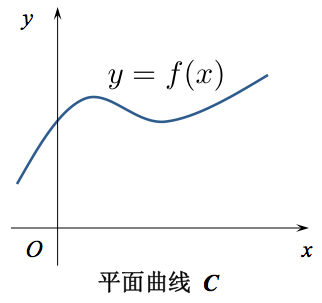
\includegraphics{./images/ch1/C_fx.jpg}}
		\end{center}\pause 
		\column{0.5\textwidth}
		\begin{center}
			\resizebox{!}{4.5cm}{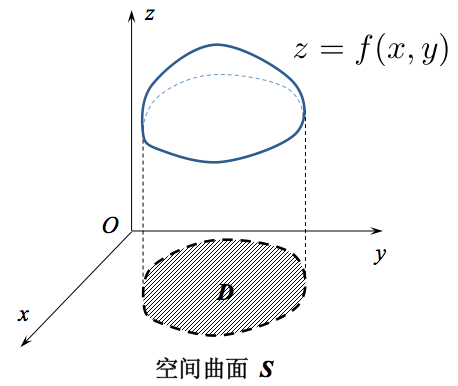
\includegraphics{./images/ch1/S_fxy.jpg}}
		\end{center}
	\end{columns}\pause 
 	\vspace{1ex}
	{\ba {问:}}平面曲线与一元函数具有一一对应关系?\pause (\alert{$\times$})
\end{frame}

\begin{frame}{一些常用的特殊函数}
	\linespread{1.2}\pause 
	\begin{enumerate}
	  \item {\bf 符号函数}\pause \\
	  $$\bm{\mathrm{sgn}}\,x\pause =\left\{
		\begin{array}{rl}
		-1,\;&x<0\pause \\
		0,\;&x=0\pause \\
		1,\;&x>0
		\end{array}
	  \right.$$\pause 
	  \item {\bf 取整函数}\pause \\
	  $$y=\left[ \,x\, \right]$$\pause 
	  $[\,x\,]$表示{\b 小于等于$x$的最大整数}
	\end{enumerate}
\end{frame}

\begin{frame}
	\linespread{1.3}
	\begin{exampleblock}{{\bf 例2:}给出以下曲线的方程}\pause
		\begin{center}
			\resizebox{!}{2.5cm}{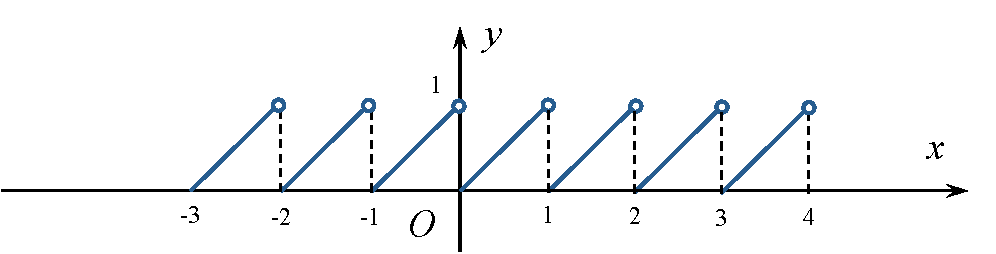
\includegraphics{./images/ch1/f1.pdf}}\\
			\pause
			\resizebox{!}{2.5cm}{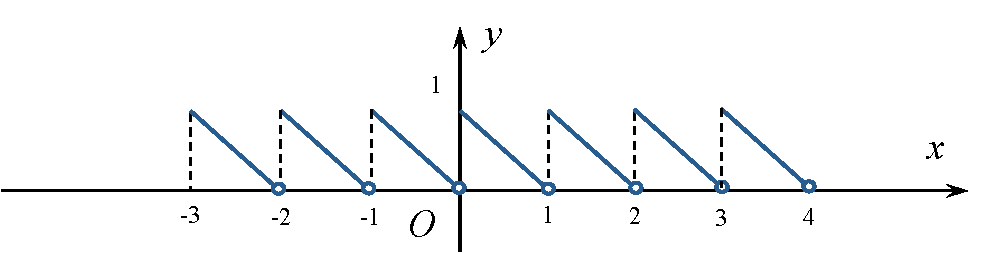
\includegraphics{./images/ch1/f2.pdf}}\\
			\pause
			\resizebox{!}{2.5cm}{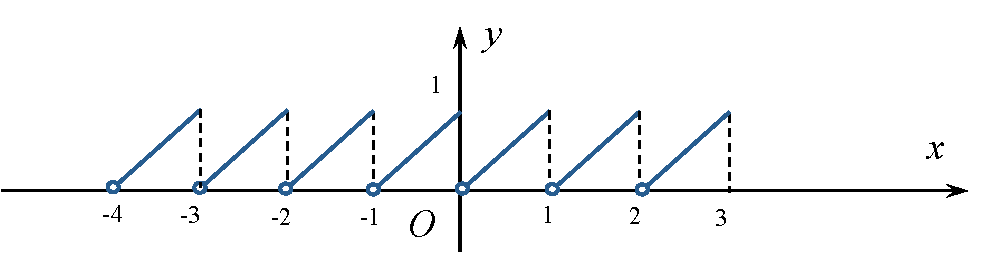
\includegraphics{./images/ch1/f3.pdf}}
		\end{center}
	\end{exampleblock}
\end{frame}

\begin{frame}
	\linespread{1.5}\pause 
	\begin{enumerate}
	  \addtocounter{enumi}{2}
	  \item {\bf Dirichlet函数}\pause \\
	  $$\bm{D}(x)\pause =\left\{
	  \begin{array}{ll}
	  	1,\;& x\in\mathbb{Q}\pause \\
	  	0,\;& x\notin\mathbb{Q}
	  \end{array}
	  \right.$$\pause 
	  \begin{itemize}
	    \item $D(x)$在实数轴上处处无极限\pause
		\item $D(x)$在实数轴上处处不连续\pause
		\item {\b 仅在一点连续的函数:}$xD(x)$
	  \end{itemize}
	\end{enumerate}
\end{frame}

\begin{frame}
	\linespread{1.5}\pause 
	\begin{enumerate}
	  \addtocounter{enumi}{3}
	  \item {\bf Riemann函数*:}\pause $(x\in[0,1])$\pause 
	  $$\bm{R}(x)\pause =\left\{
		\begin{array}{ll}
		1,\;&x=0\\\pause 
		\displaystyle\frac 1q,\;&x=\displaystyle\frac pq,\,p,q\mbox{互素}\\\pause 
		0,\;&x\notin\mathbb{Q}
		\end{array}
	  \right. $$\pause 
	  \begin{itemize}
	    \item 对任意$x_0\in[0,1]$,\pause $\lim\limits_{x\to x_0}R(x)=0$\pause 
	    \vspace{1ex}
	    \item $R(x)$在{\b 无理数点连续,\pause 有理数点不连续}
	  \end{itemize}
	\end{enumerate}
\end{frame}

\section{函数的简单性质}

\begin{frame}{函数的简单性质}
	\linespread{1.5}\pause 
	\begin{columns}
		\column{.4\textwidth}
			\begin{enumerate}
			  \item {\bf 有界性}\pause 
			  \item {\bf 单调性}\pause 
			  \item {\bf 奇偶性}\pause 
			  \item {\bf 周期性}\pause 
			\end{enumerate}
		\column{.6\textwidth}
			\begin{block}{常用数学符号}
				\begin{itemize}
				  \item {\b$\bm{\forall}$} \quad 任意 (for all) 
				  \item {\b$\bm{\exists}$} \quad 存在 (exist)
				  \item {\b$\bm{\Rightarrow}$} \quad 推出 (deduce)
				  \item {\b$\bm{\Leftrightarrow}$} \quad 等价 (equivalent)
				  \item {\b$\bm{\to}$} \quad 趋于 (approach)
				\end{itemize}
			\end{block}
	\end{columns}
\end{frame}

\begin{frame}
	\linespread{1.4}
	\begin{block}{{\bf 定义1(有界性)}}\pause 
		设函数$f:D\to\mathbb{R}$,
		\begin{enumerate}
		  \item {\bb $f(x)$有上界:}\pause $\exists$常数$M$,\pause 使得对$\forall x\in
		  D$,\pause 有 $$f(x)\leq M$$\pause
		  \vspace{-2em} 
		  \item {\bb $f(x)$有界:}\pause $\exists M>0$,\pause 使对$\forall x\in D$,\pause 有
		  $$|f(x)|\leq M$$
		\end{enumerate}
	\end{block}\pause 
	{\bf 注:}函数的有界性等价于其值域的有界性
\end{frame}

\begin{frame}
	\linespread{1.4}
	\begin{exampleblock}{{\bf 例2:}讨论如下函数的有界性}
		\quad(1)\;$y=\arctan x$,\hspace{2em}\pause (2)\;$y=e^x$,\hspace{2em}\pause
		(3)\;$y=x\sin x$\pause
	\end{exampleblock}
	\ba{“反面定义”的写法}\pause 
	\begin{enumerate}
	  \item \alert{“任意”和“存在”互换}\pause 
	  \item \alert{“$\geq(\leq)$”和“$<(>)$”互换}\pause 
	\end{enumerate}
	\begin{block}{{\bf 定义1'}(无界性)}
		设函数$f:D\to\mathbb{R}$,若对$\forall M$,$\exists x_M\in D$,使得
		$f(x_M)>M$,则称{\bb $f(x)$无上界}。
	\end{block}
\end{frame}

\begin{frame}
	\linespread{1.4}
	\begin{block}{{\bf 定义2(单调性)}}\pause 
		设函数$f:D\to\mathbb{R}$,$(a,b)\subset D$,\pause 
		{\bb $f(x)$在$(a,b)$上单调递增},是指:\pause $\forall a<x_1<x_2<b$,有
		$$f(x_1)\leq f(x_2)$$
		\pause 若上式中等号恒不成立,称{\bb $f(x)$在$(a,b)$上严格单调递增}。
	\end{block}\pause 
	\begin{exampleblock}{{\bf 例3:}讨论如下函数的单调性}
		\quad(1)\;$y=x\mathrm{sgn}(x)$\pause\hspace{3cm}(2)\;$y=x+\sin x$
	\end{exampleblock}
\end{frame}

\begin{frame}
	\linespread{1.4}
	\begin{block}{{\bf 定义3(奇偶性)}}\pause 
		设函数$f:\mathbb{R}\to\mathbb{R}$,\pause 
		{\bb 称$f(x)$为偶函数},是指:\pause 对$\forall x\in\mathbb{R}$,有
		$$f(-x)=f(x)$$
	\end{block}\pause 
	\bigskip
	\begin{exampleblock}{{\bf 例4:}试给出如下性质的数学定义}\pause
		\begin{enumerate}
		  \item 函数$y=f(x)$的图像关于$x=a$对称\pause
		  \item 函数$y=f(x)$的图像关于点$(x_0,y_0)$对称\pause
		\end{enumerate}
	\end{exampleblock}
	\alert{{\bf 思考:}$f(x)=g(a-x),\;(x\in\mathbb{R})$有什么几何意义?}
\end{frame}

\begin{frame}
	\linespread{1.4}
	\begin{block}{{\bf 定义4(周期性)}}\pause 
		设函数$f:\mathbb{R}\to\mathbb{R}$,\pause 
		称{\bb $f(x)$为周期函数},是指:\pause $\exists T>0$,
		使对$\forall x\in\mathbb{R}$,有
		$$f(x+T)=f(x).$$
		\pause 满足以上性质的最小正数$T$称为$f(x)$的{\bb 最小正周期}
	\end{block}\pause 
	\begin{itemize}
	  \item 若$T$是$f(x)$的周期,则对$\forall n\in\mathbb{N}$,$nT$也是\pause
	\end{itemize}
	$$f(x+nT)=f(x),\;(x\in\mathbb{R})$$
\end{frame}

\section{初等函数}

\begin{frame}{初等函数}
	\linespread{1.4}\pause 
	\begin{enumerate}
	  \item {\bf 幂函数:}\pause $y=x^a,\;\pause (a\in\mathbb{R})$\pause 
	  \item {\bf 指数函数:}\pause $y=a^x,\;\pause (a>0,a\ne 1)$\pause 
	  \begin{itemize}
	    \item {\b $y=e^x$}\pause 
	  \end{itemize}
	  \item {\bf 对数函数:}\pause $y=\log_ax,\;\pause (a>0,a\ne 1)$\pause 
	  \begin{itemize}
	    \item {\b$y=\ln x$}\pause 
	  \end{itemize}
	  \item {\bf 三角函数:}\pause $\sin x,\pause \,\cos x,\,\pause \tan x,\pause \,\cot
	  x,\,\pause \sec x,\,\pause \csc x$\pause 
	  \item {\bf 反三角函数:}\pause $\arcsin x,\pause \,\arccos x,\pause \arctan x,
	  \ldots$\pause 
	\end{enumerate}
	{\ba{要求:}}\pause 熟练掌握初等函数的定义、性质和相关公式
\end{frame}

\begin{frame}{其他常用函数}
	\linespread{1.2}\pause 
	\begin{enumerate}
	  \item {\bf $n$次多项式(函数):}\pause 
	  $$P_n(x)=\sum_{i=0}^na_ix^i,\pause
	  \;(a_i\in\mathbb{R},i=1,2,\ldots,n)$$\pause
	  \begin{itemize}
	    \item {\b $n$次多项式方程$P_n(x)=0$在$\mathbb{R}$上最多有$n$个根\pause (包含重根)\pause ,在
	    $\mathbb{C}$上有且仅有$n$个根(包含重根)}\pause 
	    \item {\b 设$x_i\in\mathbb{C}(i=1,2,\ldots,n)$为$P_n(x)=0$的全部根\pause ,则
	    $$P_n(x)=\prod_{i=1}^n(x-x_i)$$}\pause 
	    \vspace{-1em}
	    \item {\b 已知$P_n(x)$在$n+1$个点处的值,\pause 可以唯一确定$P_n(x)$}
	  \end{itemize}
	\end{enumerate}
\end{frame}

\begin{frame}
	\linespread{1.2}
	\begin{enumerate}
	  \addtocounter{enumi}{1}\pause 
	  \item {\bf 有理函数:}\pause 
	  $$f(x)=\frac{P(x)}{Q(x)},\pause \quad\mbox{其中}P(x),Q(x)\mbox{均为多项式函数}$$\pause 
	  \begin{exampleblock}{{\bf 例5:}用多项式除法化简以下函数}
	  	$$\frac{5x^3+3x^2+1}{x+1}$$
	  \end{exampleblock}\pause 
	  \item {\bf 双曲函数:}\pause 
	\end{enumerate}
	{\small $$\sinh x\pause =\df{e^x-e^{-x}}{2},\pause \,
	\cosh x\pause =\df{e^x+e^{-x}}{2},\pause \,\tanh x\pause=\df{\sinh
	x}{\cosh x},\pause \ldots$$}
\end{frame}

\section{曲线的参数方程}

\begin{frame}{曲线的参数方程}
	\linespread{1.2}\pause 
	\ba{问题:}$y=f(x)$能否表示平面上的所有曲线?\pause 
	\vspace{-2em}
	\begin{columns}
		\column{.45\textwidth}
			\begin{center}
				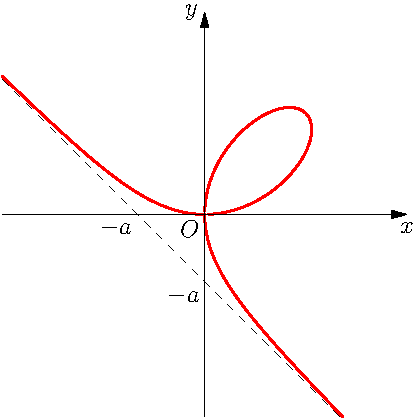
\includegraphics[width=5.5cm]{./images/ch1/dicartesCurve.pdf}
							
				{\small\bf\b Descartes叶形线}\pause
			\end{center}
		\column{.55\textwidth}
			{\small
			\bigskip
			\begin{itemize}
			  \item {\bf 参数方程:}
			  	$$\left\{\begin{array}{l}
			  		x=\df{3at}{1+t^3},\\[1em] y=\df{3at^2}{1+t^3}
			  	\end{array}\right.\;(t\in\mathbb{R})$$\pause
			  	\vspace{-1em}
			  \item {\bf 隐函数方程:}
			  	$$x^3+y^3-3axy=0$$
			\end{itemize}
			\pause
			\vspace{-1em}
			\alert{{\bf 思考:}参数方程=“含参的方程”?}
			}
	\end{columns}
\end{frame}

\begin{frame}{曲线的参数方程}
	\linespread{1.5}\pause
	\begin{exampleblock}{{\bf 例6:}求下列曲线的参数方程}
		\begin{enumerate}
		  \item 求过平面上两点$P_i(x_i,y_i)\,(i=1,2)$的直线;\pause
		  \item 半径为$a$的圆产生的圆滚线(教材P34图1.3.4)。
		\end{enumerate}
	\end{exampleblock}\pause
	\begin{itemize}
	  \item \alert{利用参数方程可以表示平面上的任意曲线}\pause
	  \item \alert{任意曲线的参数方程均不唯一}\pause
	\end{itemize}
	\bigskip
	{\bf 课后阅读:}教材P33例3。
\end{frame}

\begin{frame}{极坐标}
	\linespread{1.5}\pause 
	$$(x,y)\;\to\;(\rho\cos\theta,\rho\sin\theta)\quad\pause
	(\rho>0,\theta\in\mathbb{R})$$\pause
	\begin{exampleblock}{{\bf 例6:}求以下曲线的极坐标方程\hfill P38-例9}
		\vspace{-1ex}
		\begin{columns}
			\column{.5\textwidth}
				\begin{enumerate}
				  \item $y=kx,(k\in\mathbb{R})$
				  \item $x+y=1$
				\end{enumerate}
			\column{.5\textwidth}
				\begin{enumerate}
				  \addtocounter{enumi}{2}
				  \item $x^2+y^2=R^2,\,(R>0)$
				  \item $(x^2+y^2)^2=2a^2xy$
				\end{enumerate}
		\end{columns}
	\end{exampleblock}\pause
	\bigskip
	\alert{\bf 思考:}将极坐标方程化为平面直角方程应注意些什么?
\end{frame}

% \begin{frame}{title}
% 	\linespread{1.2}
% 	\begin{block}{title}
% 		this is sth
% 	\end{block}
% \end{frame}

\begin{frame}[<+->]{小结}
	\linespread{1.3}
	\begin{enumerate}
	  \item {\bf 函数及其性质}
	  \begin{itemize}
	    \item 有界性、单调性、奇偶性、周期性、{\b 对称性}、\ldots
	  \end{itemize}
	  \item {\bf 初等函数与常用函数}
	  \item {\bf 参数方程与极坐标方程}
	\end{enumerate}
	\pause
% 	\vspace{1em}
	\pause
	\begin{exampleblock}{课后习题}
	  \begin{itemize}
	    \item 书面作业:\\
	    {\small\b 习题1.2:3(3,4,6),7,12,13(2);习题1.3:1,5}
	    \item 思考题:\\
	    {\small\b 习题1.2:8,14-19;习题1.3:6-9;习题5.2:3}
	  \end{itemize}
	\end{exampleblock}
\end{frame}

\begin{frame}{Mathematica绘图}
	\linespread{1.4}
	\begin{exampleblock}{{\bf 例7:}画出以下方程对应的曲线}
		\begin{enumerate}
		  \item $x^3+y^3-3axy=0$
		  \item $y^2=\df{x^3}{1-x}$
		  \item $x=\sin(mt),y=\sin(nt)$
		  \item $x=\sin(nt+\sin t),y=\cos(nt+\cos t)$
		  \item $x=\cos t-\cos(nt)\sin t,y=2\sin t-\sin(nt)$
		  \item $\rho=\sin\theta+\sin^3a\theta$
		\end{enumerate}
	\end{exampleblock}
\end{frame}

\begin{frame}{课堂练习}
	\linespread{2}
	\begin{exampleblock}{{\bf 例8:}证明以下恒等式\hfill 习题5.2:3}
		\begin{enumerate}
		  \item $3\arccos x-\arccos(3x-4x^3)=\pi,\;\left(|x|\leq\df 12\right)$
		  \item $2\arctan x+\arcsin\df{2x}{1+x^2}=\pi,\;(x>1)$
		\end{enumerate}
	\end{exampleblock}
\end{frame}

\end{document}
